
%(BEGIN_QUESTION)
% Copyright 2006, Tony R. Kuphaldt, released under the Creative Commons Attribution License (v 1.0)
% This means you may do almost anything with this work of mine, so long as you give me proper credit

Suppose the liquid volume in this vessel steadily accumulates due to a constant flow rate of liquid entering the vessel through the pipe.  Graph this constant value of flow over time, given the graph of accumulating volume over time.  The function you graph (describing liquid flow) will be the {\it time-derivative} of the function shown (describing liquid volume):

$$\includegraphics[width=15.5cm]{i01529x01.eps}$$

The unit of time for the graph's horizontal axis is minutes:seconds, not hours:minutes.

\underbar{file i01529}
%(END_QUESTION)





%(BEGIN_ANSWER)

$$\includegraphics[width=15.5cm]{i01529x02.eps}$$

%(END_ANSWER)





%(BEGIN_NOTES)



%INDEX% Mathematics, calculus: derivative (calculating flow rates from measured volumes at specific times)

%(END_NOTES)


